\documentclass[a4paper,oneside,12pt,draft]{report}
\usepackage[margin=2.7cm]{geometry}
\usepackage{titlesec}
\usepackage[backend=biber]{biblatex}
\usepackage{url}
\usepackage[obeyDraft]{todonotes}
\usepackage[utf8]{inputenc}
\usepackage[acronym]{glossaries}
\usepackage[activate={true,nocompatibility},final,tracking=true,kerning=true,spacing=true,factor=1100,stretch=10,shrink=10]{microtype}
\usepackage[pdfusetitle]{hyperref}
\usepackage{pgfplots}
\usepackage{graphicx}
\usepackage{listings}
\usepackage{framed}
\usepackage{float}
\usepackage{xcolor}
\usepackage{parskip}
\usepackage{tikz}
\usepackage{dot2texi}
\usepackage{hyperref}
\usepackage[binary-units=true]{siunitx}
\usetikzlibrary{calc,positioning,arrows,chains,shapes,matrix}

\definecolor{keyword}{HTML}{008000}
\definecolor{comment}{HTML}{408080}
\definecolor{strings}{HTML}{BA2121}
\definecolor{codegray}{rgb}{0.5,0.5,0.5}

\lstdefinestyle{mystyle}{
commentstyle=\color{comment},
keywordstyle=\color{keyword},
numberstyle=\tiny\color{codegray},
stringstyle=\color{strings},
basicstyle=\footnotesize,
breakatwhitespace=false,
breaklines=true,
captionpos=b,
keepspaces=true,
numbers=left,
numbersep=5pt,
showspaces=false,
showstringspaces=false,
showtabs=false,
tabsize=2
}

\lstset{style=mystyle, language=Python}

\title{Online Event Management Software | Digital Scholarship}
\author{Jackson Chadfield}
\date{\today}

\titleformat{\chapter}{\normalfont\huge}{\thechapter.}{20pt}{\huge\bf}

\makeglossaries
\newacronym{orm}{ORM}{Object Relational Mapper}

\addbibresource{documentation.bib}

\begin{document}

	\listoftodos

	\begin{titlepage} % Suppresses displaying the page number on the title page and the subsequent page counts as page 1
		\newcommand{\HRule}{\rule{\linewidth}{0.5mm}} % Defines a new command for horizontal lines, change thickness here

		\center % Centre everything on the page

		%------------------------------------------------
		%	Headings
		%------------------------------------------------


		\textsc{\LARGE Sancta Maria College}\\[1.5cm] % Main heading such as the name of your university/college

		\textsc{\Large Digital Technologies}\\[0.5cm] % Major heading such as course name

		\textsc{\large Scholarship}\\[0.5cm] % Minor heading such as course title

		%------------------------------------------------
		%	Title
		%------------------------------------------------

		\HRule\\[0.4cm]

		{\huge\bfseries Online Event Management Software}\\[0.4cm] % Title of your document

		\HRule\\[1.5cm]

		%------------------------------------------------
		%	Author(s)
		%------------------------------------------------

		{\large\textit{Author}}\\
		Jackson \textsc{Chadfield} % Your name

		%------------------------------------------------
		%	Date
		%------------------------------------------------

		\vfill\vfill\vfill % Position the date 3/4 down the remaining page

		{\large\today} % Date, change the \today to a set date if you want to be precise

		%------------------------------------------------
		%	Logo
		%------------------------------------------------

		\vfill\vfill
		
\includegraphics[width=0.2\textwidth]{static/logo.png}\\[1cm] % Include a department/university logo - this will require the graphicx package

		%----------------------------------------------------------------------------------------
		\vfill
		% Push the date up 1/4 of the remaining page

	\end{titlepage}

	\tableofcontents
	\pagebreak

	\chapter{Preface}
	This project is my submission for the \textbf{New Zealand Technology Scholarship}\footnote{\url{https://nzqa.govt.nz/qualifications-standards/awards/new-zealand-scholarship/scholarship-subjects/scholarship-technology/}}

	It is completely open source as part of my ethos and commitment to privacy \& transparency. The source code is available on github\footnote{\url{https://github.com/j-chad/event-app}}.
	
	I have also deployed the application, which is available at \url{https://jchad-event-app.herokuapp.com/}. This online version will only be available October - December due to hosting costs. The serving of static files uses the default development server. This is inefficient but I do not have the budget to use a service such as AWS to efficiently serve these files. Thus it feels much slower than it would in a true production environment.

	This document was written in \LaTeX{} and is also freely available on the public repository.


	\chapter{Introduction}
	\todo{Change to past tense}
	I was approached by my clients, who recently had problems organising a school ball. Their main problem was communication between the large volume of attendees and the organisers. In particular, there were difficulties in efficiently notifying and updating all attendees of upcoming events and changes.

    One of the main concerns for notifying attendees was that not all attendees used just one platform such as Facebook. This meant some of the attendees were not always receiving important information.

    My clients were mostly school students that had many other obligations and were volunteering to organise the ball. They found it difficult to keep everyone updated while still studying and performing other responsibilities.

	\section{Initial Consultation}
	I met with my clients, the Ball Committee, to discuss how they previously organised the ball, problems they encountered and to discuss their ideas for improvements.

    The previous ball was organised largely through Facebook. The Ball Committee members were all administrators of the page and published updates to attendees on this platform. Students attending the ball were advised to subscribe to the facebook page. The Committee found that not all students were on Facebook. This caused a need for the information to be relayed through other mediums such as email or SMS, inducing an effect not dissimilar to Chinese whispers as information was not always relayed as intended. In effect, this created more work for the Ball Committee and meant there wasn't a single source of information.

    I asked the Committee if they could instead relay all their information by email rather than Facebook. They said most students do not regularly check their school email address, and it is harder to reply to a large volume of questions using this format. I then asked if the school newsletter would be a possible solution. However not all Teachers read out the information, and students don't tend to seek it out on their own.

    To better understand the issue, I surveyed students who were not on Facebook. I found that a large proportion of respondents were worried about the privacy implications following the recent Facebook data scandal. I then asked this group what their preferred social media platform was, of which I got a large range of different apps.

	\section{Specifications/Requirements}
	After the initial consultation and some research, the main specifications of this project are:
	\begin{itemize}
		\item Organisers can send out rich content updates that \textbf{all} users can subscribe to.
		\item Users will be able to easily find events that matter to them
		\item Notifications and updates will be presented in real time.
		\item It must be aesthetically pleasing and appealing to the target audience.
		\item Users will be able to ask questions about the event.
		\item The app must be accessible by everyone.
	\end{itemize}
	On top of these requirements, the service should also be secure, private and easy to use.

	\section{Key Stakeholders}
	My key stakeholders are the Ball Committee and those attending the school ball. My project is all about effective communication between these two parties so I need to consider their needs and feedback throughout the development process. I have arranged to meet with various Ball Committee members during development to discuss progress and future features being considered. I have decided to meet with different Committee members individually during this time, to get a better range of ideas.

	I will also be consulting fellow students about design and features to ensure that it is easy for them to use. I need to ensure I get a wide range of students in order to receive feedback that is reflective of the intended audience.

	While the Ball Committee and attendees are my key stakeholders, I am also aware that this project has the potential to cater to a much larger demographic. During the development of this project, I will also consider how it could be used in other events, such as community events and concerts.

	\section{Concept Statement}
	My stakeholders, who recently organised a school ball, have voiced concerns about the difficulty it takes to organise events with a high number of attendees. A website event management system would help to ease the burden of effective communication to large groups of attendees. While this would be developed with the stakeholders in mind, it would also be beneficial for other large events.

    The main problem I will be solving is a unified way to communicate between organisers and a large number of attendees. Key to this is to ensure that \textbf{all} attendees receive up to date reliable information in a timely and consistent manner.

	\section{Existing Solutions}
	Event management is a fairly common task so there exists a multitude of solutions that I must evaluate. This will help me to determine the strengths and weaknesses of each and give me insight on what to implement in my app.

	\subsection{Facebook Events}
	\missingfigure{Facebook events}

	\subsection{Eventbrite}
	\todo{Include client feedback}
	Eventbrite is another very popular event management system, that lets users view nearby events.
	It supports buying tickets, as well as settings to make the event private or public. The UI is a modern and clean design, and I found it very easy to navigate and create an event.

	\begin{figure}[H]
		\caption{Eventbrite Homepage}
		\includegraphics[width=\linewidth]{static/eventbrite-home.png}
	\end{figure}

	The event pages give a high amount of detail, without cluttering the screen. Including a map, and the time of the event. This will be important in my application, as the user needs to be able to quickly see the information.

	\begin{figure}[H]
		\caption{Eventbrite Event Page}
		\includegraphics[width=\linewidth]{static/eventbrite-event.png}
	\end{figure}

	A big problem with this site, is that it doesn't allow for messages to the attendees, or for the attendees to ask questions about the event, which were both part of my specifications. Additionally, the site is also full of ads and trackers, which poses a privacy concern.

	\subsubsection{Conclusion}
	The user interface of eventbrite is well designed, with clean colours and well presented information. I like the fact that it supports tickets, but I will not be implementing this due to the cost and security issues that it raises. I will, however, consider their design and flow between pages when developing my application.

	\chapter{Research}

	\section{Language}
	Each programming language has its own strengths and weaknesses. Since the programming language I use for the back end will drive the whole application, it is important to choose a language that will suit a web application. For a language to suit this project it must have a few features:

	\begin{itemize}
		\item It must be able to be concurrent and able to respond to requests simultaneously due to the large volume of users expected to use this site.
		\item It must be quick to develop in given the time constraint.
		\item It must easily and efficently interface with popular relational databases
	\end{itemize}

	I have decided to evaluate the following languages, which I have experience in: Javascript, PHP, Python and C\#.

	\subsection{Javascript}
	Javascript is a dynamic, duck-typed language. It has been the de facto language for front-end programming since the inception of the web. Recently it has also become a popular back-end language with the advent of nodejs. This gives developers the significant advantage of only having to learn and write programs in one language both client-side and server-side.

	Javascript is a relatively new language for programming the back-end, it has historically been used to write code on the front-end. In recent years it has taken off and become popular due to website designers only needing to learn one language in order to build an application. The maturity of this language as a back-end is concerning, as it may not be as heavily vetted as alternatives. There are also other quirks of the language that put me off, such as strange type coercion (1 == “1”) and implicit global variables. I have a lot of experience using this language on the front-end but very little on the back-end.

	\subsection{PHP}
	PHP is the most widely used language for web development in the world, with over 80\% of websites using it. This language does not have the problem of maturity, having been around for 24 years. The problem with PHP is it’s unpredictable and inconsistent. In PHP: NULL \(< -1\) yet NULL \(== 0\). This is not a one-off case. The whole language is riddled with strange design decisions and many ways to do a single thing, each with different naming schemes. On top of all this, the language encourages bad website design and makes you go out of your way to create secure apps.

	\subsection{Python}
	Python is an object-oriented language that has been around for almost 28 years. It is a general-purpose programming language and has many frameworks that enable web development. The syntax and language are very concise and expressive, making development very quick and easy to debug. Python avoids both the pitfalls of PHP and Javascript and is very flexible. Since python is an interpreted language it is marginally slower than similar languages which are compiled. The fact that it is not specific to web development means that I can use a wide range of tools to accomplish my tasks.
	
	\subsection{C\#}
	C\# is a strongly typed, compiled language from the C family. It was created by microsoft as an interface for .NET, a common core between many languages. Included in .NET is the ASP.NET library, the server-side web framework. The compiled nature of this language allows heavy optimisations to be made at compile time, leading to speed ups in the application. I have experience in using this language as it is used in my job for a large-scale international web application. While it works well with large applications that require constant maintenance and have a company driving development, it is generally overkill for smaller scale applications. ASP.NET development is much slower (albeit more thorough) than dynamic languages such as the above.
	
	\subsection{Conclusion}
	I have opted to use Python as the primary development language for my application. This is due to the dynamic nature of the language which allows a 
	fast development pace. As well as the large community and environment that comes with it. Using PyPI (a.k.a the Cheese Shop), I have access to over \(113,000\) packages created by the python community that can help me to develop certain features.

	\section{Web Framework}
	In order for me to efficiently and securely write a web app, I will need to use a web framework which handles all low-level details such as HTTP and routing logic, I will need to use one of the many web frameworks made for python. A web framework sits between the browser and the language and handles common logic that is general to all websites. This allows me to ignore implementation details and focus on higher level application logic. The two most common frameworks in python are \textbf{flask} and \textbf{Django}. There is a divide in the community about which is better, but the general consensus is that they are both suited for different use cases.

	\subsection{Django}
	Django is a web framework that takes a "battery included approach". It includes many features out of the box, meaning programmers can spend more time writing code without worrying about implementation details. Although this framework would have many useful features, it would impose an infrastructure that is far too heavy for my purposes. It is 180 MB which is very heavy compared to flask (6.3 MB). This is because of the "include everything" approach Django takes, whether or not those features actually get used.

	\subsection{Flask}
	Flask is a "microframework" and is the opposite of Django in the fact that it makes fewer decisions for the programmer. It is very lightweight and leaves almost all of the higher level implementation and infrastructure details to the programmer. This is perfect for my needs as I can pick and choose the features I need. Flask has a wide array of extensions made by the flask community. These range from login-management to asset bundling.
	
	\subsection{Conclusion}
	I chose to use Flask because of its scalability and extensibility. \todo{Expand web framework conclusion}

	\section{Relational Database Engine}
	\todo{Expand relational database description}
	The relational database will have an important role as being the primary data store for my application. Therefore it must be efficient and reliable so as to keep my application running smoothly.

	\subsection{SQLite}
	SQLite is a lightweight database engine that operates using database files. This means it is fast, efficient and extremely easy to set up. However, this means it doesn’t provide proper access controls. Another downside is that it only supports one write operation at any given time. The slow write operations will be a major drawback when the web app is scaled up and has many users.

	\subsection{MySQL}
	MySQL is a much more full-featured relational database. It is one of the faster available database engines available and is also one of the most popular engines. MySQL has a large open source community fixing bugs and providing support, which is always a welcome addition. MySQL is a database server (not embedded) and is designed for larger applications. MySQL is well known for being very secure and performant, both features would add value to my application. MySQL also offers a much more full-featured language with support for more constructs.

	\subsection{PostgreSQL}
	PostgreSQL is also a very popular relational database. It has very similar features to MySQL but is closer to the ANSI SQL standard, i.e. more feature complete. PostgreSQL is a little slower than MySQL and doesn’t perform as well in highly concurrent environments.
	
	\subsection{Conclusion}
	\todo{add relational database description}

	\section{Non-Relational Database Engine (Key-Value)}
	My non-relational database will be used to handle tasks and data which are not related but still must be stored. This will include data involving caching, tasks, rate-limiting and verification. I will use a key-value model for my non-relational data.

	\subsection{Memcached}
	Memcached is a popular key-value store which is extremely efficient and fast. However, it’s operations are not atomic, meaning race conditions can be created. This is a huge problem in my application, as it could have many hundred requests per second which must be handled simultaneously. Since the operations are not atomic, the data is not reliable with a high traffic.

	\subsection{Redis}
	Redis is another excellent non-relational database. Unlike Memcached, every operation is atomic meaning that when the application is scaled up and there may be a few hundred changes to the database every second, there shouldn't be any data race issues. This is very important in a highly concurrent application. Redis is every bit as fast as Memcached and supports more features, which is always nice.
	
	\subsection{Conclusion}
	\todo{Non-Relational conclusion}

	\section{Object Relational Mapper}
	An Object Relational Mapper (ORM) handles an abstraction level between the programming language and the database. This means that I can write python code that the ORM will: transform to SQL, execute the SQL, and transform any non-pythonic objects into python data types. This allows easy and safe development and enables me to use SQLite to test and MySQL in production with minimal changes in code.

	\subsection{PeeWee}
	Peewee is a lightweight ORM with a simple syntax. It is quick and suitable for smaller apps, but it lacks more complicated features. Another important consideration is the community size. PeeWee only has one major contributor, meaning patches and features will be released slowly. It also has very few resources online.

	\subsection{SQLAlchemy}
	SQLalchemy is a very stable ORM that integrates very nicely into flask using an extension. It is a very widely used ORM and I have the most experience with it. SQLAlchemy is much larger than PeeWee but offers a lot more features while maintaining simple and expressive syntax. There are 9 major contributors and it has a large online following. SQLAlchemy also offers the ability to drop down to raw SQL if needed, although this can open the application up to SQL injection vulnerabilities.
	
	\subsection{Conclusion}
	\todo{ORM Conclusion}

	\section{Task Queue}
	A task queue will become important in the later stages of my website when I need to write asynchronous code that doesn't block the current request. This will increase the time it takes for the web app to respond, and allow asynchronous events to be scheduled. \todo{Better explanation of a task queue}

	\subsection{Celery}
	Celery is a very large and full featured task queue. Due to the large community support, I started off with this task queue.
	However I quickly found it was much to complex and didn't have strong support for the flask web framework. It required a structure that
	interfered with the rest of my code and it needed many workarounds to get it to do basic things, such as send an email.

	\subsection{Redis Queue (RQ2)}
	I then tried a much more basic task queue which was designed to work with flask. This task queue was much more suited to my needs.
	I didn't have to worry about passing any app contexts around or use any hacky workarounds. As in the name, this task queue uses Redis as a message broker to store and retrieve tasks from.

	\section{Security Considerations}
	While this site doesn’t handle inherently sensitive data, it is my belief that any website should do their absolute best to provide a secure and private service. There are many aspects to consider when ensuring an app is secure, and it is nearly impossible to cover everything. However I will minimise risks and threats by using current security best practices.

	\subsection{Safe Password Storage}
	An important consideration in any application that manages passwords, is the hashing mechanism. I will use Bcrypt to hash the passwords with a random salt (per user) which is generated with the OS CSPRNG. Bcrypt performs in constant time which will mitigate timing attacks. The salt ensures that an attacker must bruteforce each password individually. They cannot find one hash and then test it against the whole database as each persons hash will be different, even if they have the same password.

	\subsection{SQL Injection}
	SQL Injection occurs when a SQL query takes malicious user input and executes it. It is a fairly easy threat to deal with, but it still one of the most common. Since I am using an ORM, SQL Injection will be (mostly) managed for me, with all input data being cleaned before a query is performed. Theoretically this should completely mitigate SQL injections as an attack vector. However, SQLAlchemy also allows using raw SQL for some operations. Raw SQL code will not be automatically cleaned by SQLAlchemy and is therefore unsafe unless it doesn’t rely on user input.

	\subsection{Cross Site Scripting (XSS)}
	XSS is very similar to SQL injection in the fact that it involves executing malicious input. XSS means a user can write malicious code that will be delivered to other users of the site. The template engine installed with flask (jinja2) is by default configured to escape any special symbols into the html equivalent, rendering any malicious inputs useless. However this setting escapes everything which adds unnecessary overhead and slows down the application, because of this speed loss, I decided to manually mark input as unsafe/safe. This is a bit riskier but is safe if handled correctly. I also opted to escape user input before it was entered into the database for items such as message text. This minimises future risk of the malicious data being presented to users.

	\subsection{Login Management}
	I initially began this project with the intention of creating my own login management system, however the complex and time consuming nature of this application meant I switched to a prebuilt solution using flask-login and flask-paranoid. Flask login integrates with SQLAlchemy and provides essential session management, where the session is stored as a cookie and verified each request. Flask-paranoid is used as a second layer of security which verifies that the users session doesn't suddenly switch to another computer, which could indicate the users session has been stolen by a malicious user.

	As an extra layer, I also added a verification email, which is sent to the users email. This helps to protect against spam and verifies that the user owns the email.

	\section{Design Research}

	\chapter{Development and Implementation}

	\section{Back-End}

	\subsection{Site Map}
	One of the first descisions I needed to make, is a map of the site. This was revised a few times, but I ended up with a decently simple map.

	\begin{center}
		\begin{dot2tex}[dot, autosize]
			digraph G {
			rankdir=LR
			node[shape=box];
			Event_Detail[label="Event Detail"];
			Create_Event[label="Create Event"];


			Index -> Login -> Dashboard;
			Index -> Register -> Dashboard;
			Dashboard -> Settings;
			Dashboard -> Create_Event;
			Dashboard -> Discover;
			Dashboard -> Event_Detail;
			Event_Detail -> Questions;
			Discover -> Event_Detail;
			}
		\end{dot2tex}
	\end{center}

	\subsection{Database Tables}
	\todo{Get a nicer database graph}
	\begin{center}
		\begin{dot2tex}[neato]
			graph G {
			rankdir=LR
			node[shape=box];
			edge[dir=both, arrowhead="crow", arrowtail="tee"];

			eventmessage -- event;
			event -- user;
			subscription -- event;
			subscription -- user;
			question -- answer;
			question -- event;
			question -- user;
			webpushtoken -- user;
			}
		\end{dot2tex}
	\end{center}

	\subsection{Application Diagram}
	\begin{center}
		\begin{dot2tex}[dot, autosize]
			digraph G {
			MySQL[shape=diamond];
			Redis[shape=diamond];
			SQLAlchemy[shape=box];
			App[shape=oval, label="Flask App"];
			Queue[shape=box, label="Task Queue"];
			Nginx[shape=box];
			Static[shape=folder];
			Push[shape=box, label="Push Server"];
			Browser[shape=oval];
			Worker[shape=box, label="Service Worker"];
			Email[shape=oval];

			Push -> Worker -> Browser;
			App -> SQLAlchemy[dir=both];
			App -> Redis[dir=both];
			SQLAlchemy -> MySQL[dir=both];
			App -> Queue;
			Queue -> Push;
			Queue -> Redis[dir=both];
			Queue -> SQLAlchemy[dir=both];
			Queue -> Email;
			App -> Nginx[dir=both];
			Nginx -> Browser[dir=both];
			Static -> Nginx;

			}
		\end{dot2tex}
	\end{center}

	\subsection{User Primary Key}
	The user table is one of the most important tables in the database, almost every table relies on it either directly or indirectly. Initially (and for most of its development) I used the users email as it's primary key. I made this decision as users all have separate emails and seems like a natural way to identify users. This works under most cases, however if a user needs to change their email, we need to change the primary key. This leads to essentially creating a new user, losing and invalidating all references to other tables. To solve this issue I simply changed the primary key and all related foreign keys to use a simple integer. I then used a unique constraint on email to ensure it is still unique.

	\subsection{Storing Messages}
	My application would be pretty pointless if it didn’t have a way to store and retrieve messages. Since I need to be able to use multiple types of messages, each with different data (e.g. text, location, file). This is a problem as I can’t store different types of data for each type of message. I solved this by specifying the type using a ENUM and the data is contained within a json field. This way, I can easily create new types of messages.

	\subsection{Determining Unread Messages}
	An important piece of data needed for the dashboard screen, is what messages the user hasn’t read. A simple solution to this problem would be to include a boolean on each message that indicates whether it has been displayed to the user. However, I found querying by this way slow and inefficient. I found a better solution would be to instead store a timestamp of when the user last loaded a specific event. I can then simply query any messages broadcast after this timestamp. If I index the message timestamps as a binary tree, I can then achieve an average lookup speed of \(O(\log n)\), which is a significant improvement on \(O(n)\).

	\begin{center}
		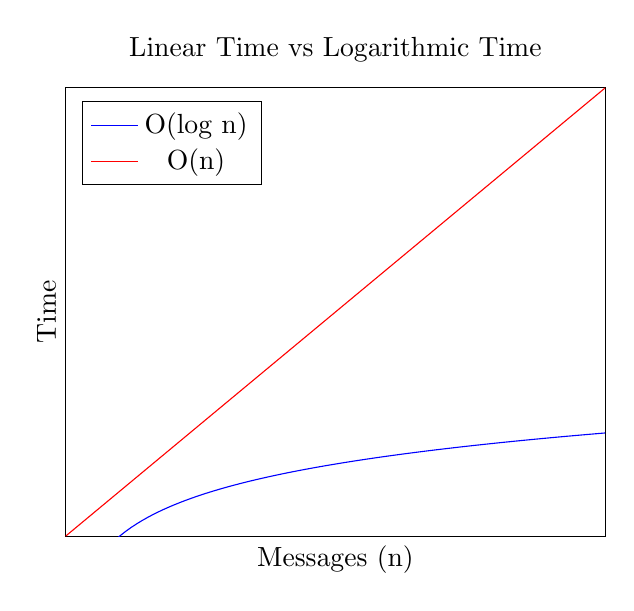
\begin{tikzpicture}
			\begin{axis}[
			title=Linear Time vs Logarithmic Time,
			xlabel=Messages ($$n$$),
			ylabel=Time,
			xmin=0,
			xmax=10,
			ymin=0,
			ymax=10,
			ytick=\empty,
			xtick=\empty,
			legend pos=north west
			]

				\addplot[
				color=blue,
				domain=0:10,
				samples=100
				]{ln(x)};
				\addlegendentry{$$O(log n)$$}
				\addplot[
				color=red,
				domain=0:10,
				samples=2
				]{x};
				\addlegendentry{$$O(n)$$}

			\end{axis}
		\end{tikzpicture}
	\end{center}

	I initially stored the “last viewed” timestamp in the redis datastore, but after some testing decided to move it to the Subscription table. This move was due to two reasons:
	\begin{itemize}
		\item The timestamp is fairly critical, we don't want the user to suddenly be notified about every single message ever sent. All critical data should be kept in the relational database.
		\item The timestamp is actually reliant on a subscription, e.g. when a user creates or deletes a subscription, the timestamp must be modified or deleted manually. This adds unnecessary code into the application and is unintuitive.
	\end{itemize}

	\subsection{Push Notifications}
	Push notifications were by far, one of the trickier features to implement. It starts off with a service worker, which must be registered in the global scope. In development, I simply set a url “/service-worker” to return the file, but in production this will be served by the web server (e.g. nginx). The user is then prompted to allow notifications. Once my app has been given permission, it will be handed some cryptographic keys and an endpoint. These are then registered in my database through an asynchronous call. I initially set the user as the primary key, however, this quickly caused errors as each endpoint is specific to a device. This meant that users would only be able to have one device receiving push notifications. I then changed the primary key to a new id column. This lead to new problems where an endpoint would be registered twice if a user subscribed, unsubscribed, and subscribed again. This caused each user to receive multiple push notifications for each event. I then attempted to solve this with a composite primary key of the endpoint and user id. This did not cause problems but on later review of the code I removed the primary key on the user id. The primary key on the user was unnecessary as each user is assigned a unique endpoint by their browser.

	\begin{center}
		\begin{figure}[H]
			\caption{Standard Push Notification Workflow}
			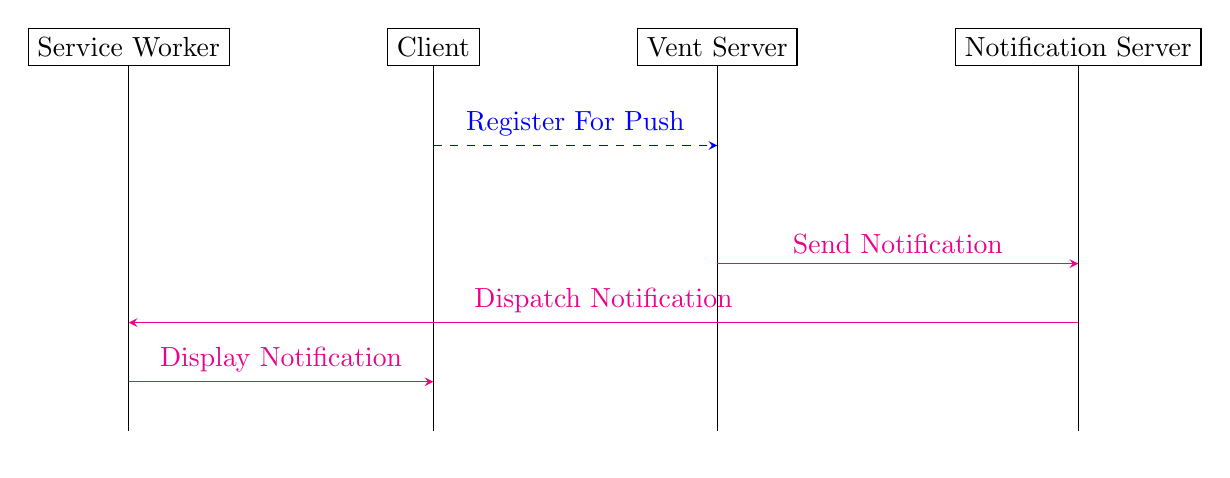
\begin{tikzpicture}[node distance=2cm,auto,>=stealth]

				\node[draw](serv_w){Service Worker};
				\node[draw, right=of serv_w](client){Client};
				\node[draw, right=of client](server){Vent Server};
				\node[draw, right=of server](notify){Notification Server};

				%Grounds
				\node[below of=serv_w, node distance=5cm](serv_w_ground){};
				\node[below of=client, node distance=5cm](client_ground){};
				\node[below of=server, node distance=5cm](server_ground){};
				\node[below of=notify, node distance=5cm](notify_ground){};

				%Draw
				\draw (serv_w) -- (serv_w_ground);
				\draw (client) -- (client_ground);
				\draw (server) -- (server_ground);
				\draw (notify) -- (notify_ground);

				\draw[->, dashed, blue]($(client)!0.25!(client_ground)$) -- node[above,scale=1,midway]{Register For Push} ($(server)!0.25!(server_ground)$);
				\draw[->, magenta]($(server)!0.55!(server_ground)$) -- node[above,scale=1,midway]{Send Notification} ($(notify)!0.55!(notify_ground)$);
				\draw[->, magenta]($(notify)!0.70!(notify_ground)$) -- node[above,scale=1,midway]{Dispatch Notification} ($(serv_w)!0.70!(serv_w_ground)$);
				\draw[->, magenta]($(serv_w)!0.85!(serv_w_ground)$) -- node[above,scale=1,midway]{Display Notification} ($(client)!0.85!(client_ground)$);

			\end{tikzpicture}
		\end{figure}
	\end{center}

	When a notification needs to be sent, a call is made to each endpoint with relevant data. I used pywebpush to achieve this. If a 410 gone or 404 not found are returned, I assume that the endpoint is expired or invalid and delete it from my database.

	\subsection{Concealing Object IDs}
	While developing the application, I realised that some of my urls weren’t as secret as they should be. The primary key for events is an integer type and is set to auto increment. This means that (most) event’s primary keys will simply be the previous event’s primary key + 1. The way that I exposed the events to users was \textbf{myapp.com/event/\textit{\textless id\textgreater}}. This gives any malicious users a straightforward way to iterate over every listed event. To fix this I used a module named hashid, which provides a reversible obfuscated base64 id. Hashids also take a salt which means its not just a straight reversal. Hashids are in no way secure, but they provide a useful url obfuscation technique.

	\subsection{GET Idempotency}
	Another issue I discovered during my development, is the method I use to access endpoints. When I added email verification to my app, I also added the ability to resend an email in case it doesn’t reach the inbox. However this method (and the logout method)  was accessed using a GET request. The issue with a GET request is that it is defined as a safe and idempotent method in the HTTP specifications. This means that it shouldn’t modify any system state, only retrieve information. Browsers will often cache and refetch endpoints retrieved with GET causing the code to run unintentionally. This could cause the user to retrieve multiple emails or be logged out without pressing anything. To fix this, I added a hidden form that is submitted when the user clicks on the logout button.

	\subsection{Password Entropy}
	When the user made a password, I wanted to ensure that it would be sufficiently secure. I began with basic password rules such as minimum length, lowercase, uppercase and digits. However I felt that this was to strict and imposing. This was also a server side validation and at the time didn’t have any client side validation. I decided to instead remove the server side validation and use a entropy + common password checker on the client side. Although it is a simple matter to bypass client side validation, there is no motivation to make a less secure password for themselves.

	\subsection{Login Lockout}
	While designing my security features, I added logic to lockout users who keep entering the wrong password in an attempt to stop brute force and dictionary attacks. I use the same identification function as my rate limiter. I also use another identification method provided by the helpful flask extension: paranoid, but paranoid tests if it is a different client, while a rate limiter checks if it is the same client. It would be extremely easy to trick paranoids detection to think you are a different user. I store the amount of times that a user has got an incorrect password in redis using the identifier. I also set an expiry time which gets reset when they get a password wrong. This allows the data to be erased after a while ensuring lockdowns are only temporary. If the number of attempts is to high, I deny any POST requests and return a helpful link to reset their password using their verified email.

	\subsection{Rich Messages}
	I wanted a simple way to enable users to write text using rich formatting. I decided on using markdown, which is a lightweight markup language, which is human readable and easy to convert to html. Converting user input into html will bring with it a risk of XSS. To circumvent this, I sanitize with \textbf{Bleach} - a library by mozilla, for sanitizing html.


	Originally, I attempted to use all messages as markdown. This lead to problems in my database. This is due to the database having max lengths for answers and questions. This can be exploited by the user by writing markdown which expands. For this reason, I decided to only use markdown for event messages.

	\begin{framed}
		For example, the markdown: \verb+* * * * * * A+ expands to \(131\) characters when converted to html. By using this technique, a \(299\) character long string can be expanded to \(> 3000\) characters.
	\end{framed}

	\lstset{language=html}
	Another problem of markdown is when it generates the HTML, it does so without context of the page it will be presented in. This means that it can (and will) generate a \lstinline|<h1>| tag in the middle of the page. This causes issues with displaying content. Luckily the markdown processor I use supports extensions, and it was a trivial matter to find an extension which increases the header depth.

	I also expanded markdown into event descriptions, to allow more control over the information presented to potential participants. This required me to change the description column from  \textit{VARCHAR(500)} to \textit{TEXT}, to avoid the problem listed above.


	\subsection{Image Messages}
	I ran into a problem when implementing sending images as messages. Traditionally images and files cannot be uploaded asynchronously, due to security risks with javascript reading local files. However, in 2008 a proposal was created for \textit{XMLHttpRequest Level 2}. This specification is an improvement on the initial \textit{XMLHttpRequest}, and allows (among many things) asynchronous file uploading. There is enough support for this standard to use it without worrying about polyfills.

	\begin{figure}[H]
		\caption{Support for XMLHttpRequest Level 2}
		\includegraphics[width=\linewidth]{static/xmlhttp2support.png}
	\end{figure}


	\subsection{Geo Search \& Mapping}
	For users to be able to see nearby events, we first need to know the location of events. An important consideration in storing the coordinates (latitude \& longitude) is how accurate they need to be. I found that 5 decimal points gives precision of ~1m which is more than enough precision. I wrote the algorithm to calculate the distance as a hybrid method in my ORM, which means it will work in the database and on the server with no changes to the code. In order to display my geographical data I needed a map provider. I initially decided on using bing maps, but after a few hours with no results, I switched to mapbox using leaflet. I was able to quickly get a map displayed using mapbox and leaflet.

	\subsection{Server to Client Communication}
	While users of my application will get real-time emails and push notifications, any updates to the data will not be presented to them until the page is refreshed. This is an important feature for my application to have, before the data is truly real-time. HTTP is traditionally a half-duplex protocol, where a client sends a request and received a response. To show real time data, I need to be able to send data to the client from the server whenever there is new data. There have been numerous methods used in an attempt to overcome these limitations. One of the most common of these methods, is simply asking the server constantly for the new data. A variation on this is asking for the data and then the server waits until it receives new data before responding. While some of these techniques work well, they have a large amount of overhead, constantly sending or receiving unnecessary data. There are two relatively new specifications that allow communication between the server and client. The first method I tried was Server Sent Events (SSE). SSE is built upon http and is fairly straightforward: The client connects to an event source, and then the server pushes data to that event source, giving the client the data. This is still technically half-duplex but the server initiates the request, rather than the client. The other specification is Websockets. Websockets are a separate protocol from http and are achieved by using an upgrade header in http. Websockets are fully duplex and very efficient. I used SSE as Websockets were much more difficult to implement safely and were overpowered for my needs.

	When implementing SSE I needed an identifier for each channel a user would subscribe to. A quick solution was to use the base64url encoded version of the users email, however this can leak the users email, even if served over https. I switched this to a sha256 hash, to better secure the information.

	\subsection{Image Processing}
	When a user uploads an image, I want to make sure that the Image is the most compressed, both to save space and bandwidth.
	A simple and effective first step is to limit the maximum size of the image. However if this is set too low, then the user might not be able to upload their images, and too high and it won't be effective. To fully optimise my bandwith and space I need to ensure that the images are compressed. To compress the image, I used JPEG compression set at 75\% quality and set the optimise flag, which does an extra pass through the image. This provided a much smaller file size with little decrease in visual fidelity. Too ensure that this doesn't caused a large delay in the request, I decided to measure the time it took to process the image. To measure this, I used the following code, with a large (\SI{1}{\mega\byte}) PNG image:

	\lstset{language=python}
	\begin{lstlisting}
		import time

		def process(f_handle):
		img = Image.open(f_handle)
		img.thumbnail((800, img_handle.height),Image.ANTIALIAS)
		img.save('test.jpg', optimize=True, quality=75)

		start = time.clock()
		with open('test.png') as f_handle:
		process(f_handle)
		print(time.clock() - start)
	\end{lstlisting}

	After running this code many times, I found that it takes around \SI{50}{\milli\second} to fully process the image. This is an acceptable timeframe, and will be percieved as instantaneous. As it doesn't take up much time or resources, I was able to process the image directly in the request context.

	\subsection{Generating Random Events}
	In order to test my website, I needed a number of events. For most of the developmental period I did this by hand, with 2 or 3 hardcoded events. This was fine but eventually I needed to scale up the ammount of events so it was more reflective of its intended use. To do this I wrote a simple factory which creates events in the database using random data. I then refactored the \textit{populate} command to create as many events as neccesary. This worked well but gave me very random names that were just random words glued together. To create more meaningful names I decided to use a simple Markov chain.

	A Markov chain is essentially a list of states with a probability of moving to another state. This gives a cheap way to mimic artificial intelligence. It is often used for the predictive text function in phone keyboards. In this usecase, it tells us if we have the letter \textbf{A} then the most probable next letter based on our data. We then randomly select a letter using the weights given by the chain. The process then repeats using the new letter. It can be made to work better by changing the number of letters used for the state.

	To get the data needed to find probablities, I used selenium to scrape over 1000 event names (almost 45000 characters). I then generated a markov chain (of order 1) and saved the state to a json file. This gave m

	\subsection{SQLAlchemy Queue Pool Overflow}
	While this isn't so much an error or a problem in my design, I thought it needed mentioning. One of the most common errors that was raised during the development of my app was:
	\begin{framed}
		\lstinline|sqlalchemy.exc.TimeoutError: QueuePool limit of size 10 overflow 10 reached|
	\end{framed}
	This is due to the nature of both flask and SQLAlchemy. Behind the scenes, SQLAlchemy creates a pool of connections. This is because it is inefficent to create and maintain a new connection whenever a new user connects. With large web apps this could easily lead to holding millions of database connections simultaneously. Instead a specific number of connections are created, these are reused by different users. If there are no connections ready in the pool, a new one will be created. If too many connections are held and a new one is requested, it will eventually timeout, giving this error.

	Attempting to replicate this behaviour when testing in a production environment was unsuccessful. As it turns out, this is because it is an issue only in a debugging environment. When flask is in debug mode, it keeps a live debugger open which keeps the connections busy. This means they cannot be recycled, and will be held open. This causes an overflow when the pool eventually tries to open more connections than allowed.

	The only real solution to this, is to raise the connection limit. This helps but merely delays the inevitable.

	\section{Front-End}
	Designing the front end was a lot more challenging to get right, as the user interface needed to feel friendly and simple, yet be able to be flexible. I started off with drawing up a mock of the home page eith my client, so that I could get a feel for the theme.

	\begin{figure}[H]
		\caption{The Initial Design}
		\includegraphics[width=\linewidth]{static/front-end1.png}
	\end{figure}

	We decided on an orange theme, with large simple blocks of content. This made it easy to understand the content quickly, and gave a modern feel. I decided to use milligram as a minimal css template, as it was small and didn't get in the way, while still noticeably improving the overall look and feel.

	It is also important that all of the pages work well with mobile, as it is a requirement that the website works the same on all devices and screen sizes. To ensure this, I implemented responsive design techniques that allowed the content to fit within the screen. For example,

	\subsection{Index Page}
	After my redesign of the index page, I mostly stuck with the initial design. I brightened the orange, changed the image, and made it feel a bit more modern.

	\begin{figure}[H]
		\caption{Revamped Index Page}
		\includegraphics[width=\linewidth]{static/front-end2.jpg}
	\end{figure}

	The resulting website is much more inviting with a functioning and responsive register form. In order to improve the user experience when they sign up, the register form first validates locally. If it is valid, the data will be submitted asynchronously to the server side. The data is then validated on the server to ensure the data is still valid. This provides a "fast-fail" experience when filling out the form, which ensures it will warn you if the data is not valid, saving a frustrating page refresh.

	\subsection{Dashboard}
	This page is the users main page, it gives an overview over all the events they own or follow. It is important that this page is clear and easy to navigate.

	\begin{figure}[H]
		\caption{Dashboard Page}
		\includegraphics[width=\linewidth]{static/front-end3.png}
		\label{fig:dashboard}
	\end{figure}

	For the dashboard, I opted for a card based approach. The left hand side of the screen gives information about subscribed events and owned events, as well as containing helpful statistics and buttons. The right hand side contains \textit{insights}, which are generated based on various contexts. For example, figure \ref{fig:dashboard} shows 2 \textit{warning} insights and 1 \textit{tip} insight. Updates to events will also be shown here. This design is highly customisable for the user, as well as being very flexible.

	\subsection{Discover}
	I Initially designed this page with a category based design, where there would be seperate categorys that would have a list of events. This was inspired by the google play store design.
	
	\begin{figure}[H]
		\caption{Intital Discover Page Design}
		\includegraphics[width=\linewidth]{static/front-end5.png}
	\end{figure}
	
	Upon consulting my clients, I was told that it was hard to use and confusing. The design also didn't scale down to a smaller device well. It was also difficult for the user to look for an event that matches criteria, as they would have no control over the categories that appear. After a redesign, the feedback I recieved was much more positive.

	\begin{figure}[H]
		\caption{Discover Page Redesigned}
		\includegraphics[width=\linewidth]{static/front-end4.png}
	\end{figure}
	
	This design was much more user friendly, in the sense that it gave users more refined choices as well as having better presentation of the data. The page uses flexboxes to scale appropriately on smaller screens, while keeping a consistent experience. It also gives users the ability to subscribe to an event without needing to first go to the event page.

	\subsection{Event View}
	It is imperative that the event details page will give as much information as possible, while still remaining easy to consume. This page is central to the whole app, and thus must be simple to use. My inital design was simple, yet it was not suited to resize to smaller devices.
	
	\begin{figure}[H]
		\caption{Inital Event Page Design}
		\includegraphics[width=\linewidth]{static/front-end6.png}
	\end{figure}
	
	My redesigned page takes elements from the initial design (such as the header), and uses the card based design I have used throughout the rest of the application. I use the dashboard layout, where there are two columns which contain the information and controls respectively. This design also lent itself to the inclusion of asynchronous http requests, as the grouped cards allow new entries to be included instantly.
	
	\begin{figure}[H]
		\caption{Event Page Redesigned}
		\includegraphics[width=\linewidth]{static/front-end7.jpg}
	\end{figure}


	\subsection{Create Event}
	
	

	\chapter{Evaluation}

	\chapter{Conclusion}

	\printbibliography

	\printglossaries
\end{document}
